\subsection{Nao Hardware}
The Nao Humanoid Platform is made by Aldebaran Robotics. 
Figure~\ref{fig:crrl_nao_coronal1} shows a picture of the Nao at the
Control/Robotics Research Lab of NYU Polytechnic School of Engineering.
The robot weighs $5.4 kg$ and has a maximum forward velocity over flat
terrain of approximately $1 \frac{m}{s}$.
It has 25 degrees-of-freedom (DoF) embodied via a 2 DoF head, two 5 DoF legs,
two 5 DoF arms, two 1 DoF hands, and a 1 DoF hip.
Figure~\ref{fig:nao_joints1} shows a diagram locating each of the joints on
the robot.
% Sonars, joint sensors, cameras, foot sensors, IMU, bumpers and buttons.
Each joint has an absolute angular position encoder, while the feet each have
four force sensitive resistors to detect ground contact.
The head has two color cameras, one that faces forward and the other that faces
downward to get a view of the terrain. The chest contains a 2-axis gyroscope and
a 3-axis accelerometer for inertial measurement, and two sonar transmitter-receiver
pairs for measuring the range to obstacles.
Figure~\ref{fig:nao_features1} shows a diagram locating the various robot sensors,
including those not listed above.
% Battery life, weight, top speed (before and after Lidar), sonar ranges, camera angles and pixels,
The sonars have a minimum range of $0.25 m$ and a maximum range of $2.55 m$.
They have a resolution of $1 cm$ and detect any obstacle within a $60^\circ$
cone. The cameras have a $1.22 Mp$ resolution, $30 Hz$ frame rate,
a horizontal field-of-view of $60.9^\circ$, and a vertical field-of-view of
$47.6^\circ$.
% CPU type and speed, RAM, storage space, USB, Ethernet, WiFi.
The robot is equipped with a 1.6 GHz Intel\textsuperscript{\textregistered}
Atom\textsuperscript{TM} CPU, 1 GB of RAM, and 2 GB of Flash memory.
It also has Gigabit Ethernet, 802.11 b/g/n WiFi, and USB 2.0. 
Nao's operating system is called NAOqi OS which is a customized version of
Gentoo Linux. Being a Linux distribution, the robot can be easily accessed
using ssh, scp, and ftp. This allows familiar command line tools to be used
to script behavior and manage services.
The robot can be natively programmed using the provided C++ or Python API.

% Ok, now briefly review what's to come in the subsubsections.
The Nao is a very feature rich platform suitable for a variety of autonomous
applications. The following sections will review specific aspects of the robot
relevant to Chapters~\ref{ch:results_navigation}~and~\ref{ch:results_crawl_gait}.


\begin{figure}
\centering
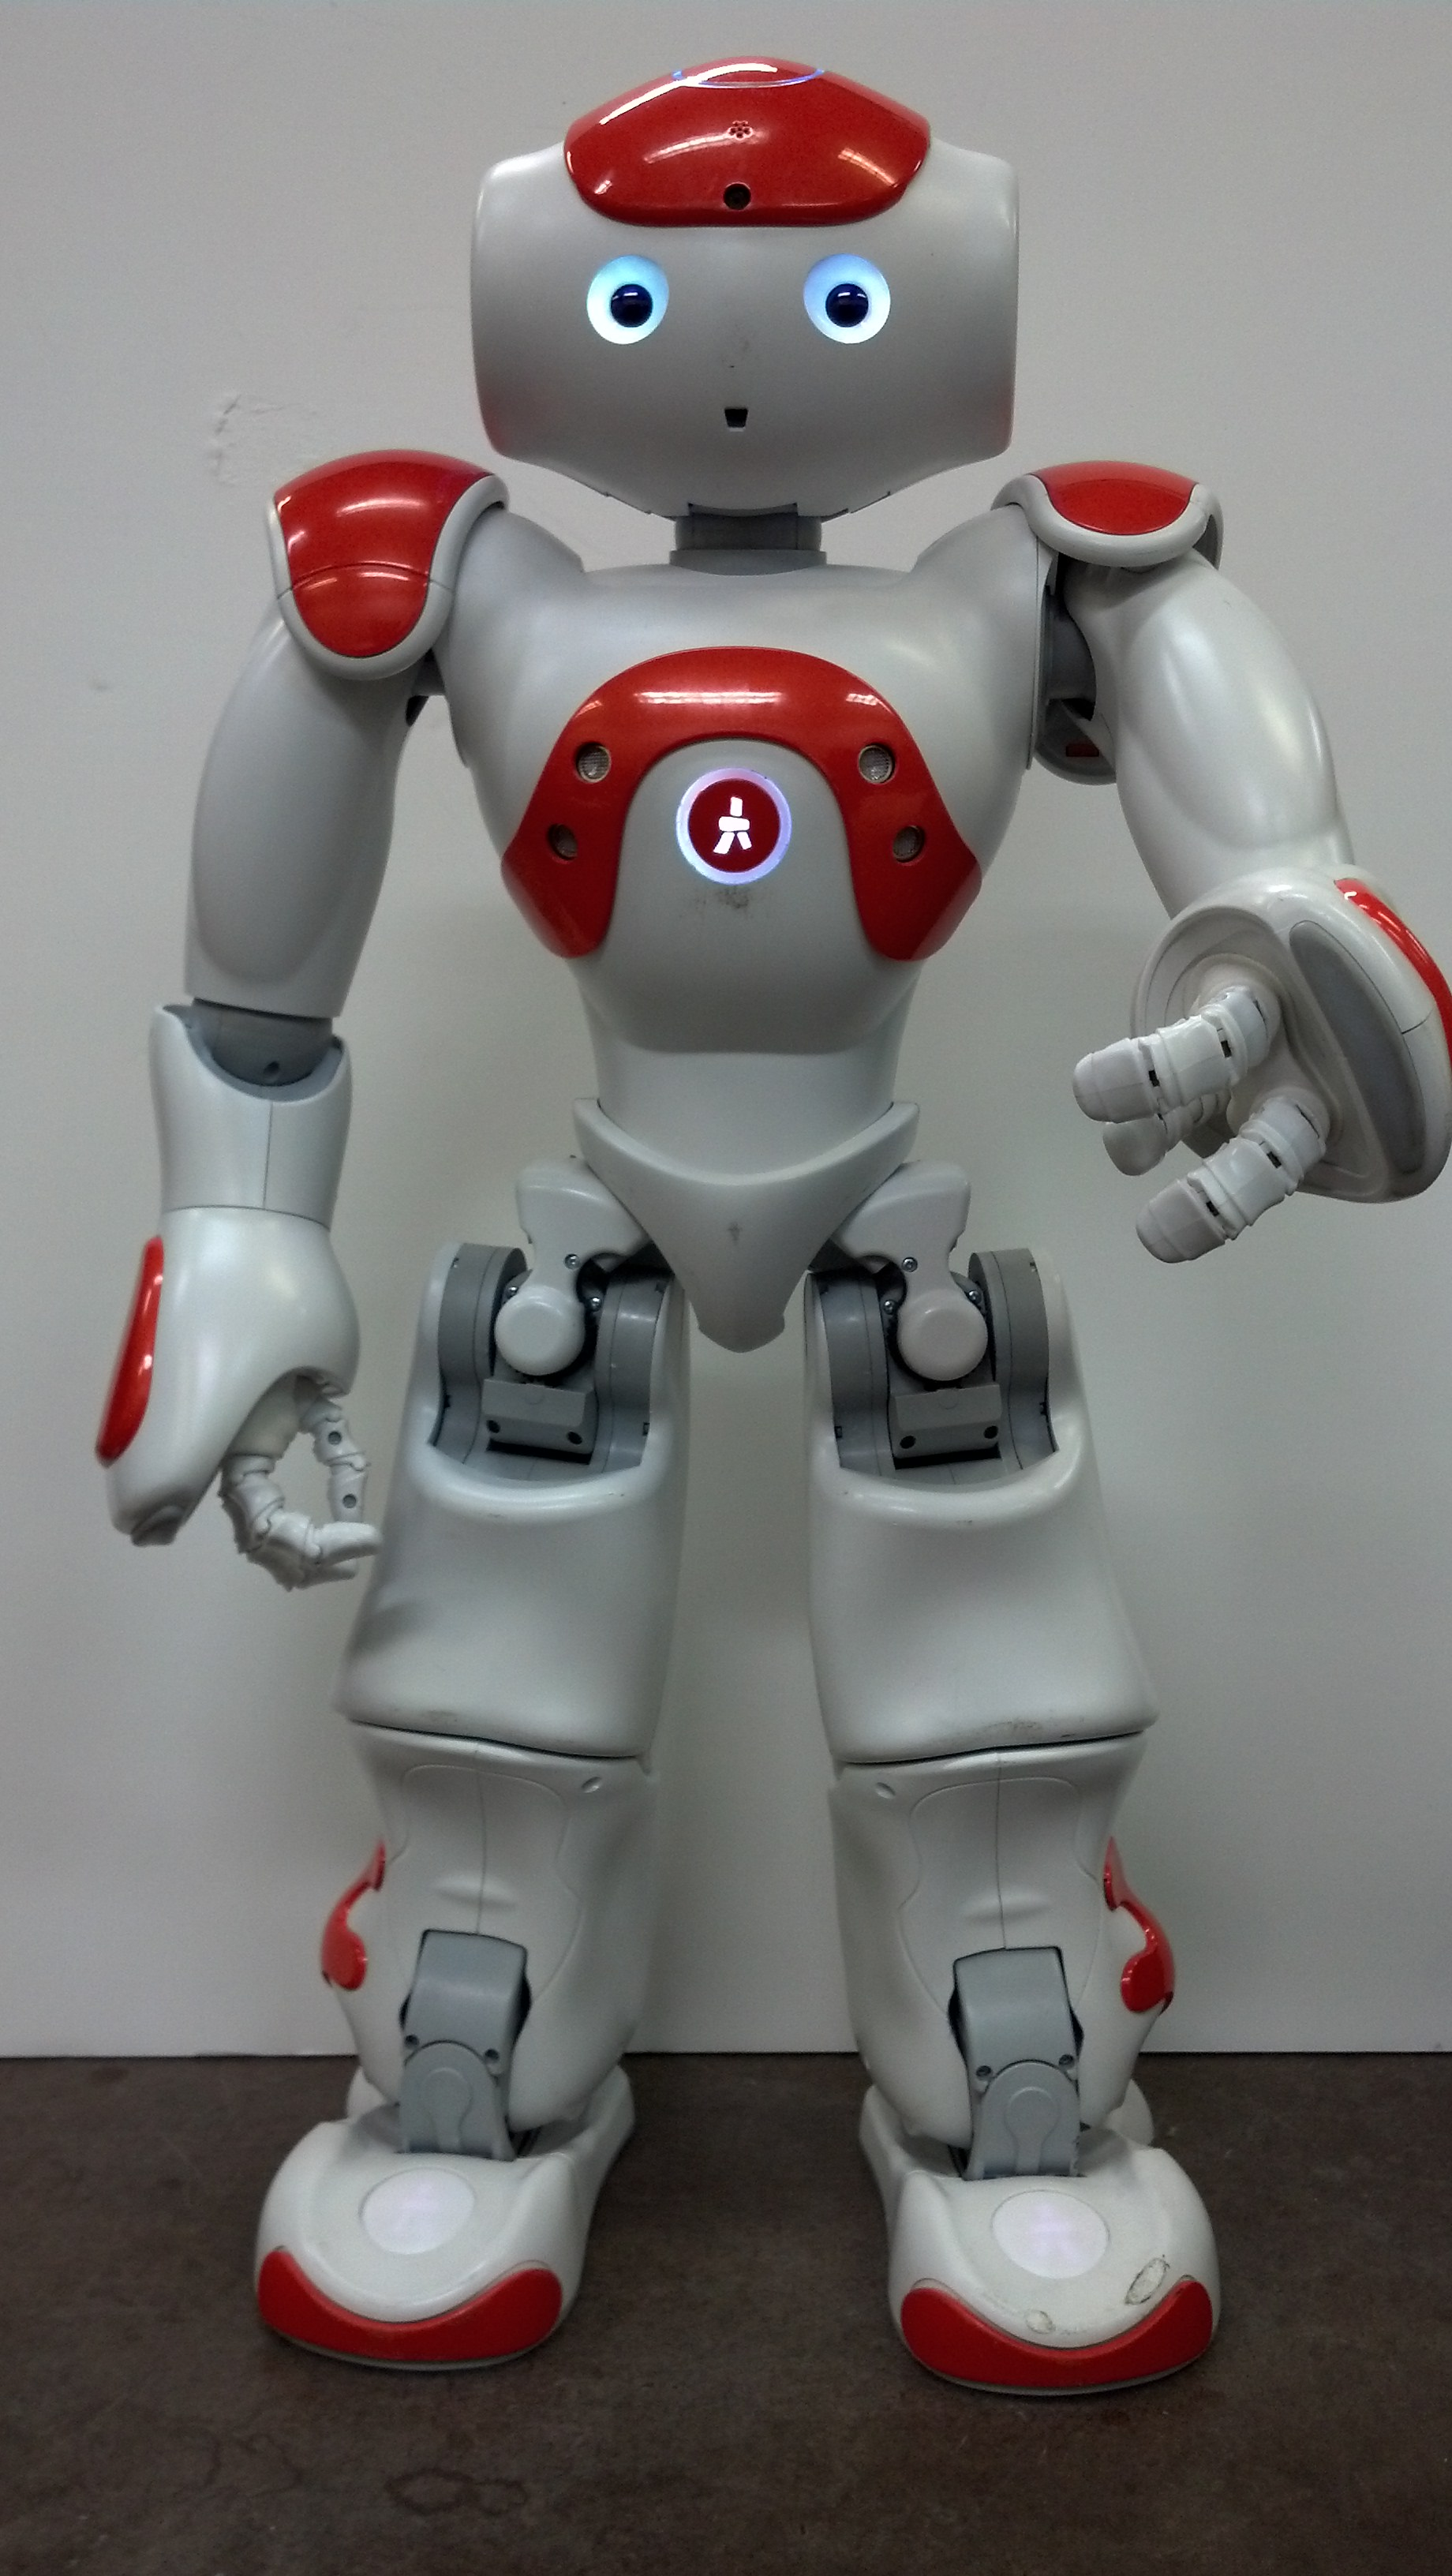
\includegraphics[height=0.4\textheight]{nao_coronal1.jpg}
\caption{Figure showing the Nao Humanoid Platform at the Control/Robotics
         Research Lab at NYU Polytechnic School of Engineering.}
\label{fig:crrl_nao_coronal1}
\end{figure}

\begin{figure}
\centering
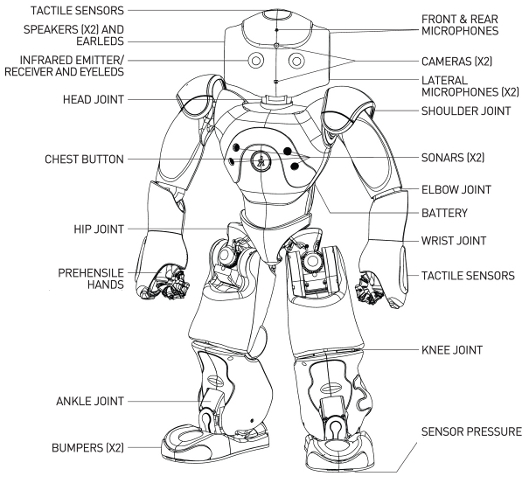
\includegraphics[width=0.4\textheight]{nao_diagrams/nao_h25_pres.png}
\caption{Figure locating the various features on the robot.}
\label{fig:nao_features1}
\end{figure}

\begin{figure}
\centering
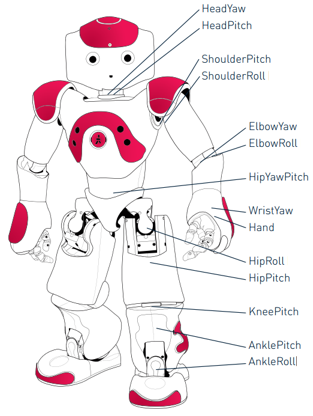
\includegraphics[height=0.4\textheight]{nao_diagrams/hardware_motortype_h25V5.png}
\caption{Figure indicating the various joint locations and their names.}
\label{fig:nao_joints1}
\end{figure}

\FloatBarrier

\subsubsection{Frame Definitions}
The NAOqi API defines three frames that can be seen in Figure~\ref{fig:nao_frames1}.
They are FRAME\_TORSO, FRAME\_ROBOT, and FRAME\_WORLD\@.
The first two frames, FRAME\_TORSO and FRAME\_ROBOT, are rigidly attached to the robot, \\
while FRAME\_WORLD is an inertial frame initialized
when the robot first starts.

\paragraph{FRAME\_TORSO} 
is a frame rigidly attached to the torso of the Nao. The positive Z-axis points
up through the head of the robot, while the positive X-axis points forwards.
It is useful for referencing different parts of the robot such and joint frames
and manipulation targets relative to the robot.
The frame origin along the X and Y directions is in the geometric center
of the torso, while Figure~\ref{fig:nao_link_lengths1} shows its Z location on
the torso as the point that the neck and hip offsets are referenced with
respect to.

\paragraph{FRAME\_ROBOT}
is a frame whose origin is between the feet of the robot. It's positive Z-axis
always points upwards and positive X-axis always points forwards. It is useful
when specifying navigation targets, relative to the Nao's current pose.

\paragraph{FRAME\_WORLD}
is a frame that is coincident with FRAME\_ROBOT when the Nao is started,
and remains static for the life of the run. It is useful for specifying navigation
and manipulation targets in a global coordinate sense.

\begin{figure}[H]
\centering
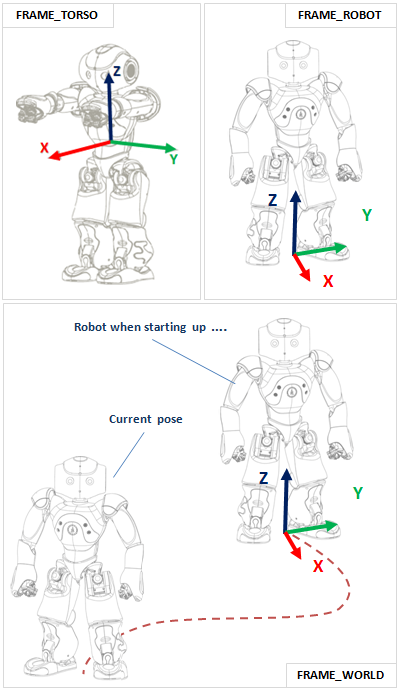
\includegraphics[height=0.75\textheight]{nao_diagrams/frame_definition_combo.png}
\caption{Nao frames.}
\label{fig:nao_frames1}
\end{figure}

Orientation targets for the Nao are commonly expressed using Tait-Bryan angles,
more commonly known as roll, pitch, and yaw. As can be seen in
Figure~\ref{fig:nao_rpy_def1}, yaw is expressed as rotation about the Z-axis,
roll is about the X-axis, and pitch is about the Y-axis.
When the robot is being referenced from the FRAME\_TORSO and is
initialized in the StandZero posture referenced in the proceeding section,
the naming conventions of the joints become clear. All joints whose axis
are parallel to the torso frame Y-axis are postfixed with the word ``Pitch'',
those parallel to the Z-axis are postfixed with the word ``Yaw'', and X-axis
with ``Roll''. The only exception to this rule is the ganged pelvis joint
axis. Each side of this degree of freedom rotates along a vector that is
in the plane formed by the torso Z-Y axes and is therefore postfixed with the
term ``YawPitch''.

\begin{figure}
\centerline{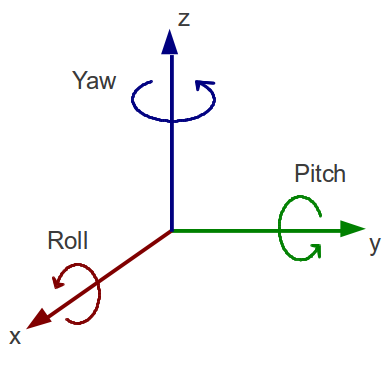
\includegraphics[width=0.5\textwidth]{nao_diagrams/rollPitchYaw.png}
}
\caption{Definition of roll pitch and yaw.}
\label{fig:nao_rpy_def1}
\end{figure}


\subsubsection{Links and Joints}
The Nao H25 is a bipedal platform with two legs, two arms, and an articulate
head. Each arm is composed of 5 joints and 3 non-zero length links, as are 
the legs. The neck is composed of 2 joints. 
There are also three fingers per hand and two feet. 
Detailed measurements and specifications on the
Nao H25 can be found on the Aldebaran Website~\cite{nao_docs_h25}.
We will review a few relevant characteristics of the robot below.

\paragraph{Links}
Figure~\ref{fig:nao_link_lengths1} shows some of the large scale link lengths
of the Nao H25. The hip and neck Z offsets are measured with respect to
FRAME\_TORSO, as are the shoulder and hip Y offsets. The thigh and tibia lengths
are each roughly $100 mm$. Their total is $202.8 mm$. The neck and hip offsets
sum to $211.5$, making the torso approximately the same length as the legs.
The humerus of the robot is nearly $100 mm$ and the forearm to the wrist
is half as long. The wrist to the hand is about half as long as the
humerus, meaning in total, the arms are about as long and the legs.

\begin{figure}
\centerline{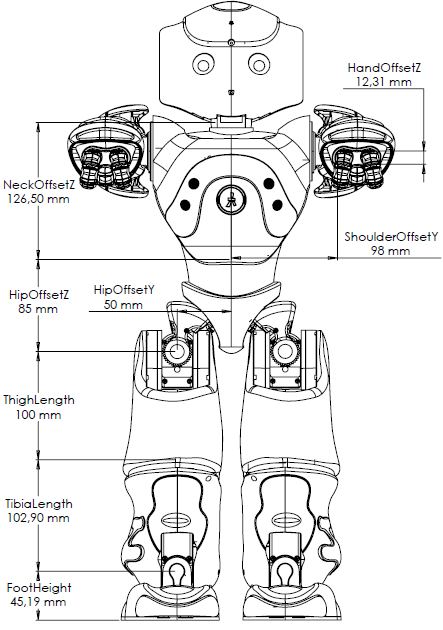
\includegraphics[width=0.45\textwidth]{nao_diagrams/hardware_lengthfront_3.3.png}
            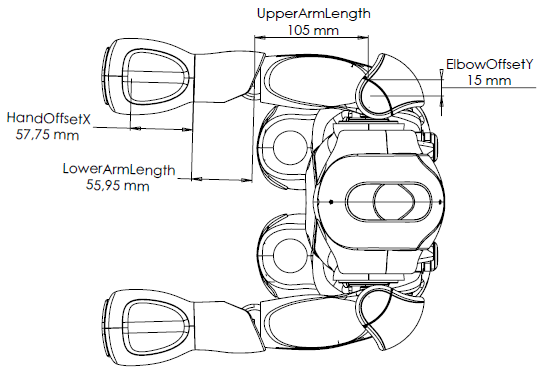
\includegraphics[width=0.55\textwidth]{nao_diagrams/hardware_lengthup_3.3.png}
}
\caption{Nao link lengths.}
\label{fig:nao_link_lengths1}
\end{figure}

\paragraph{Joints}
The Nao H25 has 25 degrees-of-freedom. Each of the two hands constitute one degree
of freedom even though each hand has 8 rotary joints. This is because they are
mechanically linked through a single actuator that pulls a cable to close the
fingers. The hand opens again through relaxation of the cable which allows springs
to extend the fingers. This means the Nao can hold its hand closed, but not open.
The two pelvis joints are mechanically linked, resulting in one degree
of freedom. A diagram of the pelvis can be seen in Figure~\ref{fig:nao_hip_yawpitch1}.
The result is the robot can spread or close both legs, but not an
individual leg. This makes certain crawling techniques inaccessible to this
body configuration.
The 22 remaining joints are each independently actuatable and constitute the
remaining degrees-of-freedom. Each leg and arm have 5 joints while the neck has
two. As shown in Figure~\ref{fig:nao_neck_joints1}, one neck joint is for pitch
and the second for yaw.
Figures~\ref{fig:nao_arm_joints_left1}~and~\ref{fig:nao_arm_joints_right1}
detail the arms which have a shoulder joint for both pitch and roll, an elbow
joint for both roll and yaw, and a wrist joint for yaw.
Figures~\ref{fig:nao_leg_joints_left1}~and~\ref{fig:nao_leg_joints_right1}
detail the legs which have a hip joint for both pitch and roll, a knee joint
for pitch, and an ankle joint for both pitch and roll.
Table~\ref{tab:joint_chains} shows the order in which each joint appears
in their respective kinematic chains.
%This needs to be said.
%In the below diagrams, the green line represents the nominal zero, the blue line
%is the min angle, and the red line is the max angle

Figures~\ref{fig:nao_neck_joints1}~through~\ref{fig:nao_hip_yawpitch1},
show the range of rotation for each joint. The joints are shown in their positions
representing zero angle. The green line is a reference representing the zero.
The red line represents the maximum angle the joint can actuate to, while the
blue line is the minimum angle.

Each joint contains a magnetic rotary encoder for measuring angular position.
These encoders have a $0.1^\circ$ precision. A motor current sensor for each
joint can also be read to get a sense of how much torque each joint is
producing, though in practice this reading is a poor approximation as it is
influenced by other factors such as motor control loop methodology.

\begin{figure}
\centering
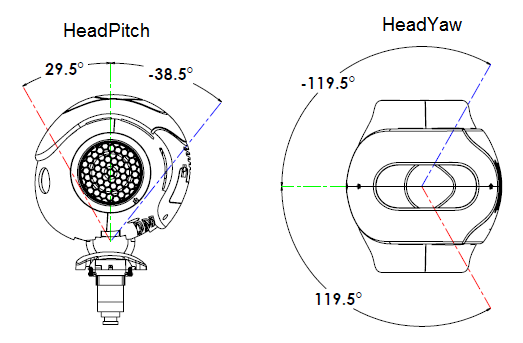
\includegraphics[width=\textwidth]{nao_diagrams/hardware_headjoint_3.3.png}
\caption{Diagram of the angular ranges of the neck joints in degrees.}
\label{fig:nao_neck_joints1}
\end{figure}

\begin{figure}
\centering
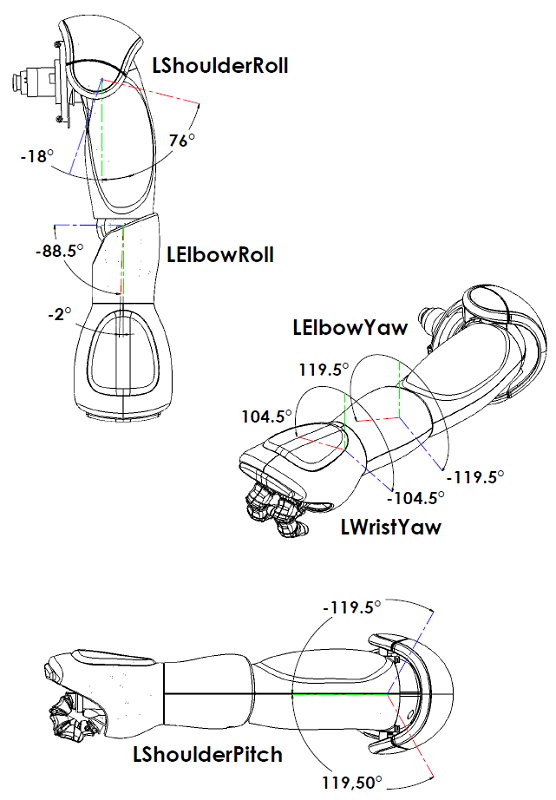
\includegraphics[width=\textwidth]{nao_diagrams/hardware_larmjoint_3.3_corr1.png}
\caption{Diagram of the angular ranges of the left arm joints in degrees.}
\label{fig:nao_arm_joints_left1}
\end{figure}

\begin{figure}
\centering
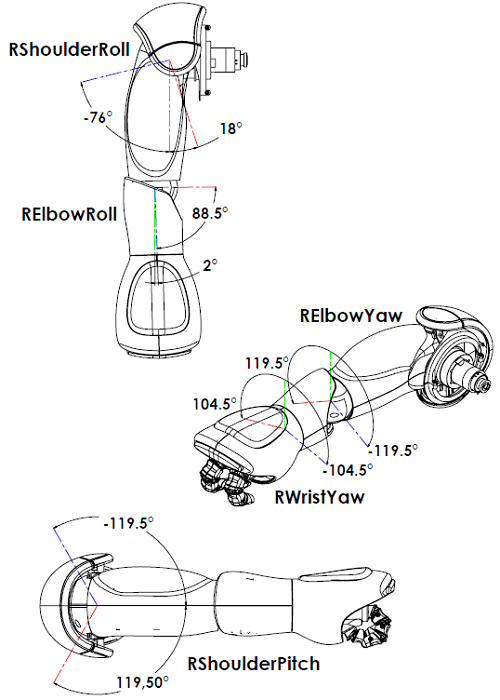
\includegraphics[width=\textwidth]{nao_diagrams/hardware_rarmjoint_3.3.png}
\caption{Diagram of the angular ranges of the right arm joints in degrees.}
\label{fig:nao_arm_joints_right1}
\end{figure}

\begin{figure}
\centering
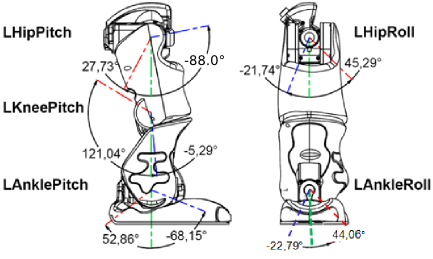
\includegraphics[width=\textwidth]{nao_diagrams/hardware_llegjoint.png}
\caption{Diagram of the angular ranges of the left leg joints in degrees.}
\label{fig:nao_leg_joints_left1}
\end{figure}

\begin{figure}
\centering
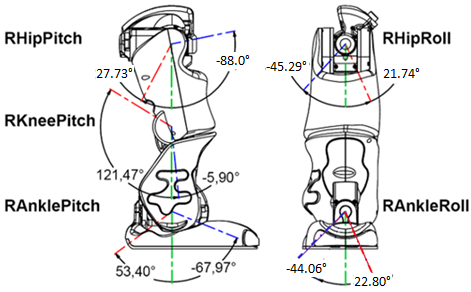
\includegraphics[width=\textwidth]{nao_diagrams/hardware_rlegjoint.png}
\caption{Diagram of the angular ranges of the right leg joints in degrees.}
\label{fig:nao_leg_joints_right1}
\end{figure}

\begin{figure}
\centering
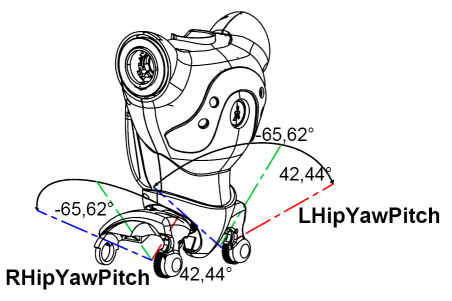
\includegraphics[width=\textwidth]{nao_diagrams/hardware_pelvisjoint.png}
\caption{Diagram of the angular ranges of the pelvis joints in degrees.
         While there are two joints, they are mechanically linked such that
         when actuated, the joints are at the same angular position.}
\label{fig:nao_hip_yawpitch1}
\end{figure}

\begin{table}
\centering
\begin{tabulary}{\textwidth}{|l||l|}
\hline
\textbf{Chain}& \textbf{Joints}\\	\hline\hline
Head	   & HeadYaw $\rightarrow$ HeadPitch    \\	\hline
Left Arm   & LShoulderPitch $\rightarrow$ LShoulderRoll $\rightarrow$ LElbowYaw $\rightarrow$ \\
           & LElbowRoll $\rightarrow$ LWristYaw   $\rightarrow$ LHand       \\	\hline
Right Arm  & RShoulderPitch $\rightarrow$ RShoulderRoll $\rightarrow$ RElbowYaw $\rightarrow$ \\
           & RElbowRoll $\rightarrow$ RWristYaw   $\rightarrow$ RHand       \\	\hline
Left Leg   & LHipYawPitch   $\rightarrow$ LHipRoll      $\rightarrow$ LHipPitch $\rightarrow$ \\
           & LKneePitch $\rightarrow$ LAnklePitch $\rightarrow$ LAngleRoll  \\	\hline 
Right Leg  & RHipYawPitch   $\rightarrow$ RHipRoll      $\rightarrow$ RHipPitch $\rightarrow$ \\ 
           & RKneePitch $\rightarrow$ RAnklePitch $\rightarrow$ RAngleRoll  \\	\hline 
\end{tabulary} 
\caption{Nao H25 kinematic chains that stem from the torso.
         Each row lists the sequence of joints for that chain.}
\label{tab:joint_chains}
\end{table}

\FloatBarrier

\paragraph{Joint Rotation Direction}
While each joint has a positive and negative angular limit, the direction
of each joint is not relative to the previous joint frame, but rather the
torso frame. This can be seen most clearly in Figure~\ref{fig:nao_arm_joints_reflect1},
which is a diagram showing the arms side-by-side, highlighting the roll joints.
It shows that positive joint angle in the roll joints always corresponds to moving to the
left side of the robot, if all other joints are in the zero position.
Negative joint angle always moves roll joints to the right. This is in contrast
to other conventions which might hold that positive roll angle might move
the joints ``outward'' or ``inward''.
As usual, joint angle frames are attached to joints and not the torso frame.
This means that if the right arm's elbow yaw joint rotated by a positive
$90^\circ$ and all other joints are at zero angle, positive elbow roll
would now correspond to the joint pitching upwards, as the elbow yaw joint
precedes the roll joint in the kinematic chain. Figure~\ref{fig:nao_postures1}
shows that when all joints are in their zero positions, the arms point forwards.

\begin{figure}
\centering
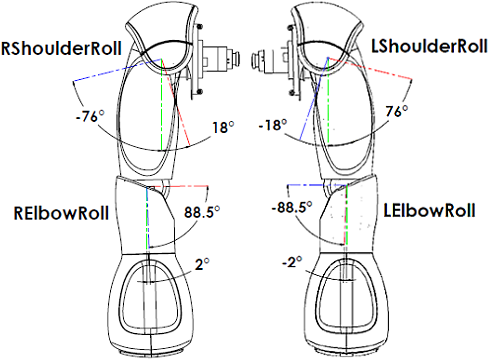
\includegraphics[width=\textwidth]{hardware_r_and_l_armjoint_corr1.png}
\caption{Figure showing arm joints and how they are a reflection.}
\label{fig:nao_arm_joints_reflect1}
\end{figure}

\FloatBarrier

\subsubsection{Joint Torques}
% Motor torques. (Important for Chapter~\ref{ch:crawl_gait})
% Talking about the joint motor torques, tables, gearboxes, blah.
The actuators for each joint are sized according to their expected capacity
requirements. The leg joints, for example, use motors with high torque as they
are expected to counteract the forces seen due to walking. This is in contrast
to the hand actuator motors which aren't required to have large grasp force
as the Nao is not rated to move heavy objects.
Table~\ref{tab:joint_motors} lists the different motors with their rated torques
used in each of the joints. Table~\ref{tab:joint_gears} lists the gearboxes
used in each actuator while Table~\ref{tab:joint_motor_gear} lists which
motor and actuator used in each joint. These figures are taken from the 
Aldebaran Website~\cite{nao_docs_h25}.

\begin{table}
\centering
\begin{tabulary}{\textwidth}{|l||l|l|l|l|}
\hline
\textbf{Motor Type}     & 1               & 2               & 3                & 4               \\ \hline
\textbf{Model}	        & 22NT82213P      & 17N88208E       & 16GT83210E       & DCX16S01GBKL651 \\ \hline
\textbf{No Load Speed}  & $ 8,300 rpm $   & $ 8,400 rpm $   & $ 10,700 rpm $   & $ 12,700 rpm  $ \\ \hline
\textbf{Stall Torque}   & $ 68 mNm $      & $ 9.4 mNm $     & $ 14.3 mNm $     & $  22.4 mNm  $  \\ \hline
\textbf{Nominal Torque} & $ 16.1 mNm $    & $ 4.9 mNm $     & $ 6.2 mNm $      & $ 5.53 mNm $    \\ \hline
\end{tabulary} 
\caption{Various parameters for each of the motors used in the joint actuators.}
\label{tab:joint_motors}
\end{table}

\begin{table}
\centering
\begin{tabulary}{\textwidth}{|l||l|l|l|l|}
\hline
\textbf{Motor Type} & 1       & 2      & 3       & 4      \\ \hline
\textbf{Ratio A}    & 201.3   & 50.61  & 150.27  & 150.27 \\ \hline
\textbf{Ratio B}    & 130.85  & 36.24  & 173.22  &        \\ \hline
\end{tabulary} 
\caption{Speed reduction gear ratios used in the joint actuators.
         Each motor type has a two different gear ratios that can be used with
         it in the joint actuator, ratio A or B.}
\label{tab:joint_gears}
\end{table}

\begin{table}
\centering
\begin{tabulary}{\textwidth}{|l||l|l|l|}
\hline
\textbf{Chain}  &  \textbf{Joint}  & \textbf{Motor Type}  & \textbf{Ratio}  \\ \hline\hline
\textbf{Head}   &                  &                      &                 \\	\hline
                & HeadYaw          & 3                    & A               \\	\hline
                & HeadPitch        & 3                    & B               \\	\hline
\textbf{Arms}   &                  &                      &                 \\	\hline
                & ShoulderPitch    & 3                    & A               \\	\hline 
                & ShoulderRoll     & 3                    & B               \\	\hline 
                & ElbowYaw         & 3                    & A               \\	\hline 
                & ElbowRoll        & 3                    & B               \\	\hline 
                & WristYaw         & 2                    & A               \\	\hline 
\textbf{Hands}  &                  &                      &                 \\	\hline 
                & Hand             & 2                    & B               \\	\hline 
\textbf{Legs}   &                  &                      &                 \\	\hline
                & HipYawPitch      & 1                    & A               \\	\hline 
                & HipRoll          & 1                    & A               \\	\hline 
                & HipPitch         & 1                    & B               \\	\hline 
                & KneePitch        & 1                    & B               \\	\hline 
                & AnklePitch       & 1                    & B               \\	\hline 
                & AnkleRoll        & 1                    & A               \\	\hline 
\end{tabulary} 
\caption{Actuator configuration for each joint consisting of motor type and gear reduction ratio.}
\label{tab:joint_motor_gear}
\end{table}

\subsubsection{Postures}
% Talking about the different postures of the robot.
The NAOqi API contains a module called ALRobotPosture which allows the robot
to be commanded to any one of a number of predefined kinematic configurations,
called ``postures''.
These postures are shown in Figure~\ref{fig:nao_postures1}.
The robot can be commanded to transition to these postures in two different ways.
Trivially, the first method is that the robot can command its joints to go 
directly to the joint angles corresponding to each posture. This is convenient
in situations where robot safety is not a factor, such as tests or initializations.
More interestingly, the second method is the robot can plan its transition
from its current joint configuration to the commanded posture in a way that
avoids self collision and prevents the robot from endangering itself, such
as when the robot might fall over. This can involve the robot first transitioning to intermediate
postures or executing maneuvers that ensure robot stability.
One example is when the robot is standing and is commanded to the ``Sit''
posture. In this scenario, the Nao will place its right hand on the ground
behind it in order to prevent itself from falling over as it moves its legs.
Using this planning paradigm, it can be commanded to any posture from any
joint configuration safely.
This feature is particularly useful when planning a full navigation sequence
and is used in Chapter~\ref{ch:crawl_gait} to transition the robot from 
walking to crawling.
\begin{figure}
\centerline{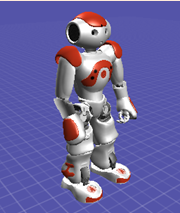
\includegraphics[width=0.33\textwidth]{posture/posture_stand.png}
            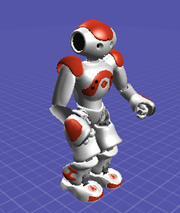
\includegraphics[width=0.33\textwidth]{posture/posture_standinit.png}
            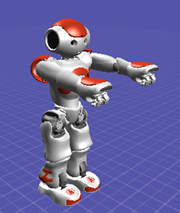
\includegraphics[width=0.33\textwidth]{posture/posture_standzero.png}
}
\vspace*{0.05in}
\centerline{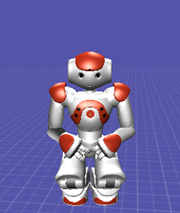
\includegraphics[width=0.33\textwidth]{posture/posture_crouch.png}
            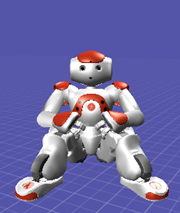
\includegraphics[width=0.33\textwidth]{posture/posture_sit.png}
            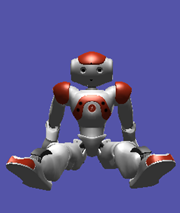
\includegraphics[width=0.33\textwidth]{posture/posture_sitrelax.png}
}
\vspace*{0.05in}
\centerline{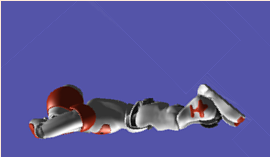
\includegraphics[width=0.5\textwidth]{posture/posture_lyingbelly.png}
            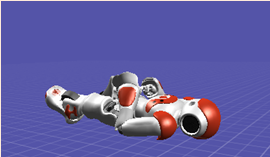
\includegraphics[width=0.5\textwidth]{posture/posture_lyingback.png}
}
\caption{Posture options for the Nao H25. From the upper left pane to the lower
         right pane they are: Stand, StandInit, StandZero, 
                              Crouch, Sit, SitRelax,
                              LyingBelly, LyingBack.}
\label{fig:nao_postures1}
\end{figure}
